\documentclass[a4paper]{article}

\usepackage{mathrsfs}
% ============================================
%         General Packages
% ============================================
\usepackage{balance}

\usepackage{kotex}      % for Korean
\usepackage{lipsum}     % for dummy text
\usepackage{array}

\usepackage{cite}   % for citation

\usepackage{amsmath,amsfonts}
\usepackage{amssymb}
\usepackage{soul}
\usepackage{mathrsfs}

\usepackage{hyperref}

    \hypersetup{
        pdftoolbar=false,        	% show Acrobat’s toolbar?
        pdfmenubar=false,        	% show Acrobat’s menu?
        pdffitwindow=false,     	% window fit to page when opened
        pdfstartview={FitH},    	% fits the width of the page to the window
        pdftitle={},    	% title
        pdfauthor={},     	% author
        %     pdfsubject={},   	% subject of the document
        %     pdfcreator={},   	% creator of the document
        %     pdfproducer={}, 	% producer of the document
        %     pdfkeywords={keyword1, key2, key3}, % list of keywords
        %     pdfnewwindow=true,      	% links in new PDF window
        colorlinks=true,       	% false: boxed links; true: colored links
        linkcolor=blue,          	% color of internal links (change box color with linkbordercolor)
        citecolor=blue,       	% color of links to bibliography
        filecolor=blue,      	% color of file links
        urlcolor=blue		% color of external links
    }

\usepackage{algorithm}
\usepackage{algorithmic}

\usepackage{epsfig}
\usepackage[dvipsnames]{xcolor}

% MY PACKAGES ===================================

\usepackage{svg}
\usepackage{subfig}

\usepackage{textcomp}
\usepackage{stfloats}
\usepackage{url}
\usepackage{verbatim}
\usepackage{graphicx}
\usepackage{multirow}
\usepackage{multicol}

\let\proof\relax
\let\endproof\relax
\usepackage{amsthm}
\usepackage{lipsum}
\usepackage{tikz}

% 
\usepackage{titlepic}
\usepackage{pdfpages}
\usepackage{etoolbox} % 조건문을 쓰기 위한 패키지


\titlepic{%
  
\includegraphics[height = 8mm]{figures/logo_KAIST_simple.png}
  \hspace{5mm}
  
\includegraphics[height = 8mm]{figures/MIC_Logo.png}
  }

% ========================================
%         TITLE and AUTHORS
% ========================================
\title{
  Nonstationary Infinite-Horizon OCP
}

\author{
    Geunyoung Park
    \thanks{\href{https://kaist-mic-lab.github.io/members/gyPark/}{Geunyoung Park} is Postdoctoral Researcher at KAIST, {\tt\small geunyoung.park@kaist.ac.kr}}%
    , and
    Seunghun Jang
    \thanks{\href{https://kaist-mic-lab.github.io/members/shJang/}{Seunghun Jang} is Ph.D. student at KAIST, {\tt\small shjang7071@kaist.ac.kr}}%
}

\date{
    % 20\textsuperscript{th} March 2025
    Complied on \today
}

\begin{document}

\maketitle

% ========================================
%         Contents
% ========================================

\begin{figure}[h]
  \centering
  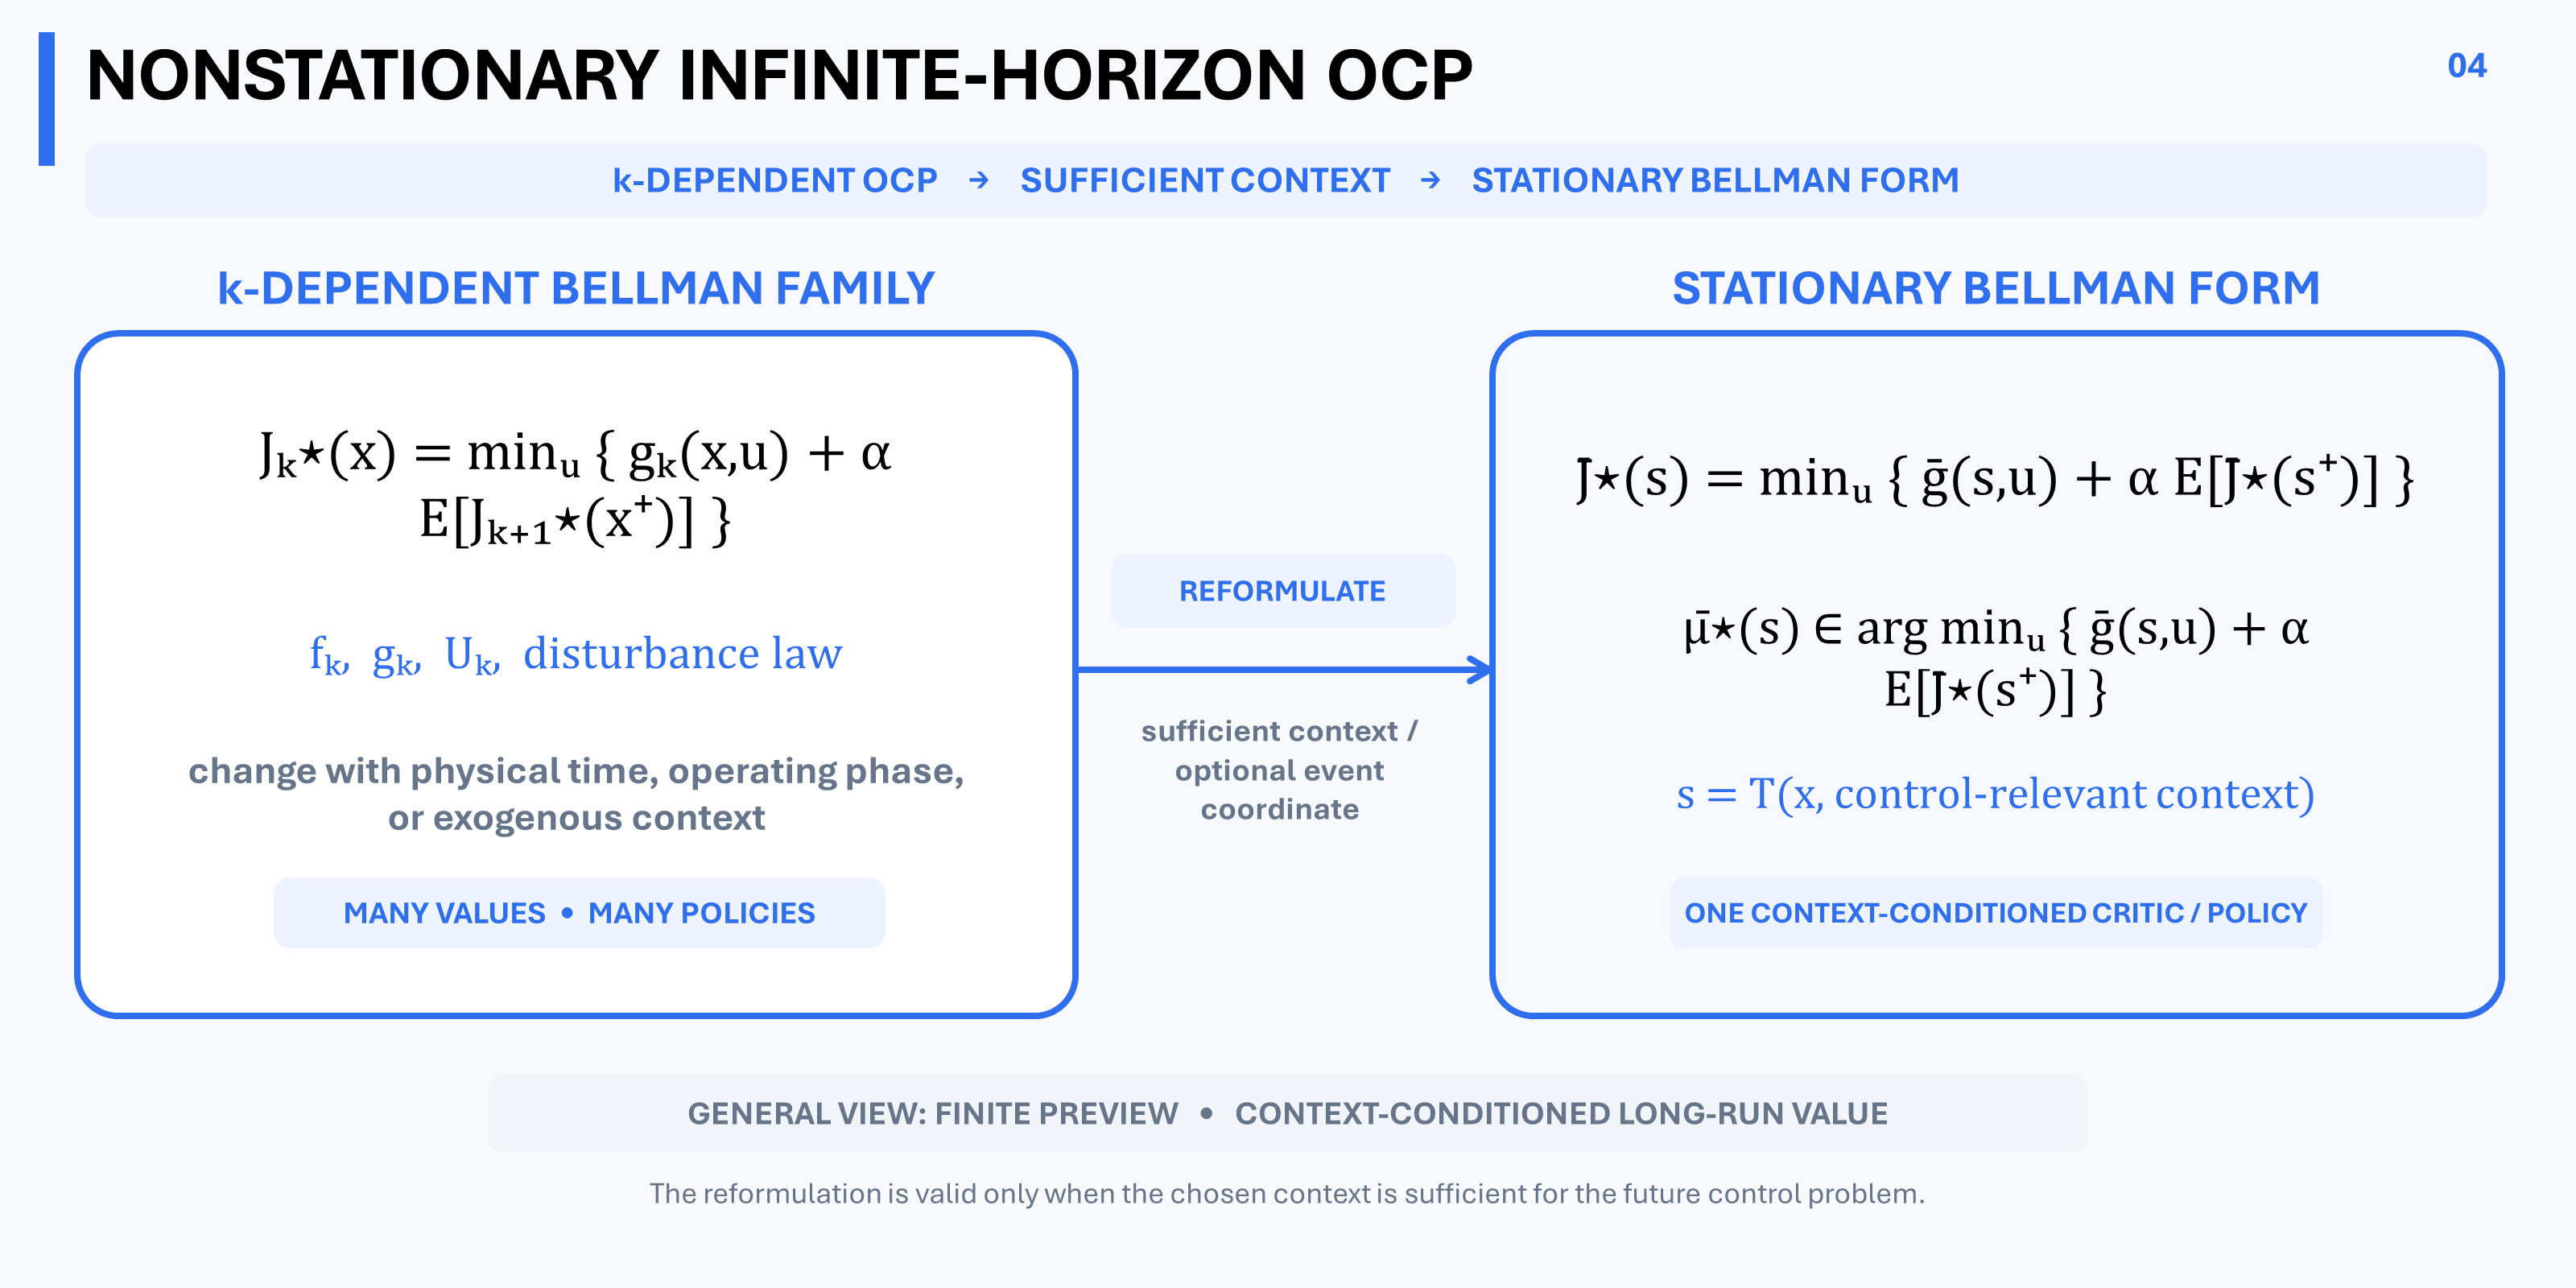
\includegraphics[width=\textwidth]{figures/04_nonstationary_infinite_horizon_ocp.png}
  \caption{A k-dependent Bellman problem is transformed, when a sufficient context exists, 
into a stationary Bellman problem on a reformulated state.}
  \label{fig:}
\end{figure}

\nocite{*} % <------------ 인용있으면 삭제

The main formulation uses a discounted infinite-horizon objective with
$0<\alpha<1$. A stationary reformulation is a research condition to be
established, not an assumption that every nonstationary problem can be
converted.

\section{Problem definition}

\href{https://kaist-mic-lab.github.io/research/research_themes/00_online_learning_based_optimal_control/}{Online Learning-Based Optimal Control} uses a stationary Bellman equation when the decision state, dynamics, stage cost, constraints, and uncertainty law are time homogeneous. Many mobility problems are instead written with explicit dependence on physical time, position within an operating profile, mission phase, operating mode, or exogenous context:

\begin{equation}
  x_{k+1}=f_k(x_k,u_k,w_k),
  \qquad
  u_k\in\mathcal U_k(x_k),
\end{equation}

with incurred stage cost $g_k(x_k,u_k)$. Here $w_k$ is the exogenous
disturbance and $\mathcal U_k(x_k)$ is the time-dependent admissible input
set.

Let $\Pi_{k:\infty}$ be an admissible class of causal state-feedback policy
sequences, with $u_\ell=\mu_\ell(x_\ell)$. The explicit index on $\mu_\ell$
allows known time dependence. When additional observed context is needed, it
is included in the decision state as in Section 5. The time-indexed optimal
value is

\begin{equation}
  J_k^\star(x)
  :=
  \inf_{\mu_{k:\infty}\in\Pi_{k:\infty}}
  \mathbb E
  \!\left[
  \left.
  \sum_{j=0}^{\infty}
  \alpha^j
  g_{k+j}(x_{k+j},u_{k+j})
  \right|
  x_k=x
  \right],
\end{equation}

with Bellman recursion

\begin{equation}
  \begin{aligned}
    J_k^\star(x)
    &=
    \min_{u\in\mathcal U_k(x)}
    \left\{
    g_k(x,u)
    +
    \alpha
    \mathbb E
    \!\left[
    J_{k+1}^\star(x^+)
    \mid x,u,k
    \right]
    \right\},\\
    \mu_k^\star(x)
    &\in
    \arg\min_{u\in\mathcal U_k(x)}
    \left\{
    g_k(x,u)
    +
    \alpha
    \mathbb E
    \!\left[
    J_{k+1}^\star(x^+)
    \mid x,u,k
    \right]
    \right\}.
  \end{aligned}
\end{equation}

Here $x^+$ denotes the successor state. The dynamic-programming principle does
not require stationarity: a nonstationary finite-horizon recursion is anchored
by a terminal condition, while the infinite-horizon version is a time-indexed
Bellman family. Its validity requires a well-posed discounted limit---such as
bounded costs with an appropriate boundedness or transversality
condition---and the future sequence of models, costs, constraints, or its
probabilistic law.

Because $f_k$, $g_k$, $\mathcal U_k$, or the disturbance law can change with
$k$, a single $J^\star(x)$ and $\mu^\star(x)$ generally cannot represent the
exact optimum. An approximate or robust stationary policy may still be useful
under declared conditions. The exact recursion is nevertheless a coupled
sequence of Bellman equations, not one stationary fixed-point equation. If
the $k$-dependence is unknown or drifting rather than known in advance or
generated by an observed Markov context, the recursion is not directly
implementable. The research problem is then to determine whether its
control-relevant cause can be represented as part of a sufficient decision
state.

\section{Why this problem matters}

In predictive control, the reference, demand, constraints, dynamics, or
disturbance statistics may vary with operating phase and available preview. A
critic trained only on physical state $x$ may then assign the same value to
two situations that share $x$ but face different future opportunities,
constraints, or costs. This \textbf{context aliasing} can prevent a stationary
policy defined on $x$ alone from representing the exact optimum, although an
approximate or robust policy may remain useful under stated conditions.

Finite-preview receding-horizon control can exploit the currently available
prediction, but it does not by itself represent the continuation beyond that
preview or recurring operation under future contexts. A valid stationary
reformulation could support a reusable long-run critic and terminal value
while retaining the context required for correct decisions.

Some apparent nonstationarity is therefore a state-representation problem: if
a finite-dimensional Markov context captures all relevant $k$-dependence and
evolves under a time-homogeneous law, the augmented problem is stationary. If
no such context exists, or its transition law itself drifts, the original
time-indexed problem remains nonstationary.

\section{Key challenges}

\begin{itemize}
  \item \textbf{Sufficient context and equivalence:} the selected
  reference-generator, operating-phase, environment, mode, or task variables
  must preserve feasible decisions, causality, and accumulated cost without
  requiring the complete history.
  \item \textbf{Coordinate or event aggregation:} changing from time samples
  to phases, segments, cycles, or decision events can lose within-event
  information; aggregated transitions, costs, constraints, and discounting
  must preserve the original problem.
  \item \textbf{Dimension and coverage:} a richer augmented state increases
  value-learning complexity and requires data across the relevant contexts.
  \item \textbf{Changing context statistics:} a critic built for a fixed
  transition law can become invalid under distribution shift; convergence on
  the reformulated model does not prove that the reformulation remains
  correct.
\end{itemize}

\section{A conventional approach — finite-preview predictive control}

An exact treatment retains the $k$ index and computes the family
$\{J_k^\star,\mu_k^\star\}$. Over an unbounded horizon this is rarely reusable
or computationally practical. A common alternative solves an $H$-stage
problem using the model, cost, constraints, and forecasts available at the
current decision time:

\begin{equation}
  V_{k,H}^{\mathrm{pred}}(x)
  =
  \inf_{\pi_{k:k+H-1}\in\Pi_{k,H}}
  \mathbb E
  \!\left[
  \left.
  \sum_{j=0}^{H-1}
  \alpha^j
  g_{k+j}(x_{k+j},u_{k+j})
  +
  \alpha^H V_{f,k+H}(x_{k+H})
  \right|
  x_k=x
  \right],
\end{equation}

subject to the predicted $k$-dependent dynamics and constraints. Here
$\Pi_{k,H}$ is a declared class of causal finite-horizon policies; each policy
maps the information available at its prediction stage to $u_{k+j}$.
Deterministic MPC commonly reduces this to an input-sequence optimization. The
controller applies the first action and repeats the problem in
receding-horizon fashion as new state and preview information become
available.

If the task truly terminates after $H$ stages with a valid terminal condition,
the finite-horizon formulation can be exact. For continuing operation, its
quality depends on the forecast, prediction horizon, and terminal
approximation $V_{f,k+H}$; a fixed $V_f$ is a special case. Unless the
terminal term correctly represents the continuation, the controller can remain
short-sighted beyond the preview window. A context-free terminal target can
also be inappropriate when slow, stored, or resource states should be
preserved differently under different future contexts. Finite-preview control
is therefore a practical baseline, not by itself a solution to the original
nonstationary infinite-horizon problem.

\section{Research direction — context- or event-based stationary reformulation}

\textbf{Context-augmented stationary form.} First preserve the physical
decision index $k$. Suppose an observed or predictable context $c_k$ and
augmented state $z_k=(x_k,c_k)$ can be constructed such that

\begin{equation}
  \Pr
  \!\left(
  z_{k+1}\mid z_{0:k},u_{0:k}
  \right)
  =
  \overline P
  \!\left(
  z_{k+1}\mid z_k,u_k
  \right),
\end{equation}

and the stage cost and feasible set admit time-independent representations:

\begin{equation}
  g_k(x,u)
  =
  \overline g\!\left((x,c_k),u\right),
  \qquad
  \mathcal U_k(x)
  =
  \overline{\mathcal U}\!\left((x,c_k)\right).
\end{equation}

The context may be an operating phase, mode, reference-generator state,
exogenous Markov state, or another finite sufficient statistic of the
available preview. Merely appending the absolute clock does not provide a
useful reusable representation unless the resulting context and its future
law are compact, time homogeneous, and learnable.

The stationary Bellman problem on the augmented state is

\begin{equation}
  \begin{aligned}
    \overline J^\star(z)
    &=
    \min_{u\in\overline{\mathcal U}(z)}
    \left\{
    \overline g(z,u)
    +
    \alpha
    \mathbb E
    \!\left[
    \overline J^\star(z^+)\mid z,u
    \right]
    \right\},\\
    \overline\mu^\star(z)
    &\in
    \arg\min_{u\in\overline{\mathcal U}(z)}
    \left\{
    \overline g(z,u)
    +
    \alpha
    \mathbb E
    \!\left[
    \overline J^\star(z^+)\mid z,u
    \right]
    \right\}.
  \end{aligned}
\end{equation}

For an augmented decision state, write $J_k^\star(x;c)$ and
$\mu_k^\star(x;c)$ for the value and policy conditional on observed context
$c$. Under an exact sufficient reformulation,

\begin{equation}
  J_k^\star(x;c_k)
  =
  \overline J^\star(x,c_k),
  \qquad
  \mu_k^\star(x;c_k)
  =
  \overline\mu^\star(x,c_k).
\end{equation}

The semicolon makes the currently observed context explicit. When $c_k$ is a
deterministic function of $k$, this reduces to the earlier notation
$J_k^\star(x)$ and $\mu_k^\star(x)$. Thus one critic exists on $(x,c)$, not on
$x$ alone. Under the well-posedness conditions in Section 1, value iteration
or approximate DP can target this critic only if the augmented transition law
is stationary and the chosen context is Markov-sufficient over the declared
operating domain.

\textbf{Optional event-coordinate form.} When decisions naturally occur at
phases, tasks, segments, or other events, the problem may instead be
re-indexed at event boundaries. Let $z$ be the augmented boundary state, $a$
an event-level decision, $G$ the discounted cost accumulated until the next
boundary, and $D$ the corresponding duration in physical steps. The essential
Bellman form is

\begin{equation}
  \overline J_{\mathrm{ev}}^\star(z)
  =
  \min_{a\in\mathcal A_{\mathrm{ev}}(z)}
  \mathbb E
  \!\left[
  G
  +
  \alpha^D\overline J_{\mathrm{ev}}^\star(z^+)
  \mid z,a
  \right].
\end{equation}

Here $\mathcal A_{\mathrm{ev}}(z)$ is the admissible event-decision set, and
$a$ may be one action or a declared causal policy within the event. The
conditional law of $(G,D,z^+)$ given $(z,a)$ must be time homogeneous, and the
aggregation must preserve within-event feasibility and path constraints. A
fixed discount per event is not equivalent when $D$ varies. Under exact
aggregation, the boundary value agrees with the original time-indexed value at
the same physical boundary.

\textbf{Use as a terminal value.} Once an exact or approximate stationary
long-run critic is available, it can replace the generic terminal
approximation $V_{f,k+H}$ in the finite-preview predictive controller of
Section 4. With an exact reformulation, model,
constraints, terminal critic, and optimization, its first action is
Bellman-consistent with the infinite-horizon optimum. An approximate critic
does not provide that guarantee automatically. This is the connection to
\href{https://kaist-mic-lab.github.io/research/research_themes/02_online_multistep_lookahead/}{Online Multistep Lookahead}:
the present Theme asks when a reusable stationary terminal-value problem
exists, whereas lookahead addresses online action improvement using a fixed
critic.

\section{Application domains}

\begin{itemize}
  \item \textbf{Forecast-driven predictive control:} represent recurring
  reference, demand, disturbance, constraint, or environment patterns through
  a sufficient context so that a finite-preview controller can use a reusable
  continuation value.
  \item \textbf{Periodic or mission-phase control:} augment the physical state
  with a finite phase or operating-mode variable when it is Markov-sufficient.
  This can replace separate time-indexed policies with one stationary critic
  and policy across recurring drive cycles, duty cycles, or mission phases.
  \item \textbf{Event-based and networked decisions:} re-index control at task
  phases, service events, road segments, charging nodes, or other decision
  boundaries. The event model must preserve accumulated cost, constraints, and
  physical duration.
  \item \textbf{xEV energy and thermal management:} the 2026 ASCC FCEV study
  is one concrete application in which road links provide event coordinates
  and a long-run network-conditioned value supplies continuation beyond the
  finite prediction window. This example motivates, but does not define, the
  general Research Theme.
\end{itemize}

\section{References}

\begin{itemize}
  \item
    \href{https://kaist-mic-lab.github.io/members/khChoi/}{Kyunghwan Choi},
    ``\href{https://kaist-mic-lab.github.io/publications/2026-traffic-network/}{Traffic
    Network-Aware Energy Management for FCEVs: Integrating Trip-Specific
    Control and Long-Run Optimality},''
    \textit{Asian Control Conference (ASCC)}, 2026.
    \href{https://kaist-mic-lab.github.io/static/pub/2026-traffic-network.pdf}{Full text}
\end{itemize}

% ========================================
%         Appendix
% ========================================

% \begin{appendices}
% \end{appendices}

\addcontentsline{toc}{chapter}{Bibliography}
\bibliographystyle{IEEEtran}
\bibliography{refs}

\end{document}
